\chapter{Projeto do Algoritmo Iterativo}
\label{cap:iterativo}

No Capítulo \ref{cap:modelagem}, uma Busca em Profundidade foi utilizada para enumerar os conjuntos viáveis no exemplo proposto. Essa abordagem, possui elevada complexidade computacional e, por isso, não representa um bom candidato a ser implementado. Nesse capítulo, o algoritmo projetado será a primeira alternativa a essa abordagem.

O algoritmo introduzido aqui é composto por três partes básicas: codificação/decodificação, busca, e ``poda''. Ao reunir esses elementos, obtém-se um método iterativo para enumerar os conjuntos viáveis. Cada uma dessas partes será detalhada antes da descrição do algoritmo ser apresentada. Ao final, será feita uma análise de sua complexidade e comparação com o desempenho da abordagem anterior. 

\section{Representando Combinações Usando Inteiros}
\label{section:codificacao}

\subsection{Codificação}

A primeira abstração a ser feita é considerar as combinações de enlaces como números binários. Nesses números, cada {\it bit} está relacionado à pertinência de um enlace específico àquela combinação. Consequentemente, também é possível representar a combinação de enlaces como um número inteiro sem sinal resultado da conversão do número na base 2 para a base 10. A seguir, essa modelagem é apresentada fazendo uso de uma linguagem mais formal, visando permitir algumas manipulações matemáticas importantes ao funcionamento do algoritmo.

Seja o grafo direcionado $G=(V,E)$. As m arestas em E são enumeradas como $e_0, e_1, e_2, ..., e_{m-1}$. Seja $B$ um número inteiro na base 2 com $m$ {\it bit}s. Os {\it bit}s em $B$ são enumerados como $b_0, b_1, b_2, ..., b_{m-1}$. Seja uma combinação de arestas $C$ tal que $C \in E$. O número $B$ codifica a combinação $C$ quando:

\[ b_i =
\begin{cases}
	1	\text{, sse } e_i \in C\\
	0	\text{, caso contrário}\\
  \end{cases}
\]

Essa ideia de codificação é estendida para toda a árvore de combinações. Ao fazer isso, todos os $2^m$ vértices da árvore serão codificados em inteiros.

\begin{figure}[htb]
\centering
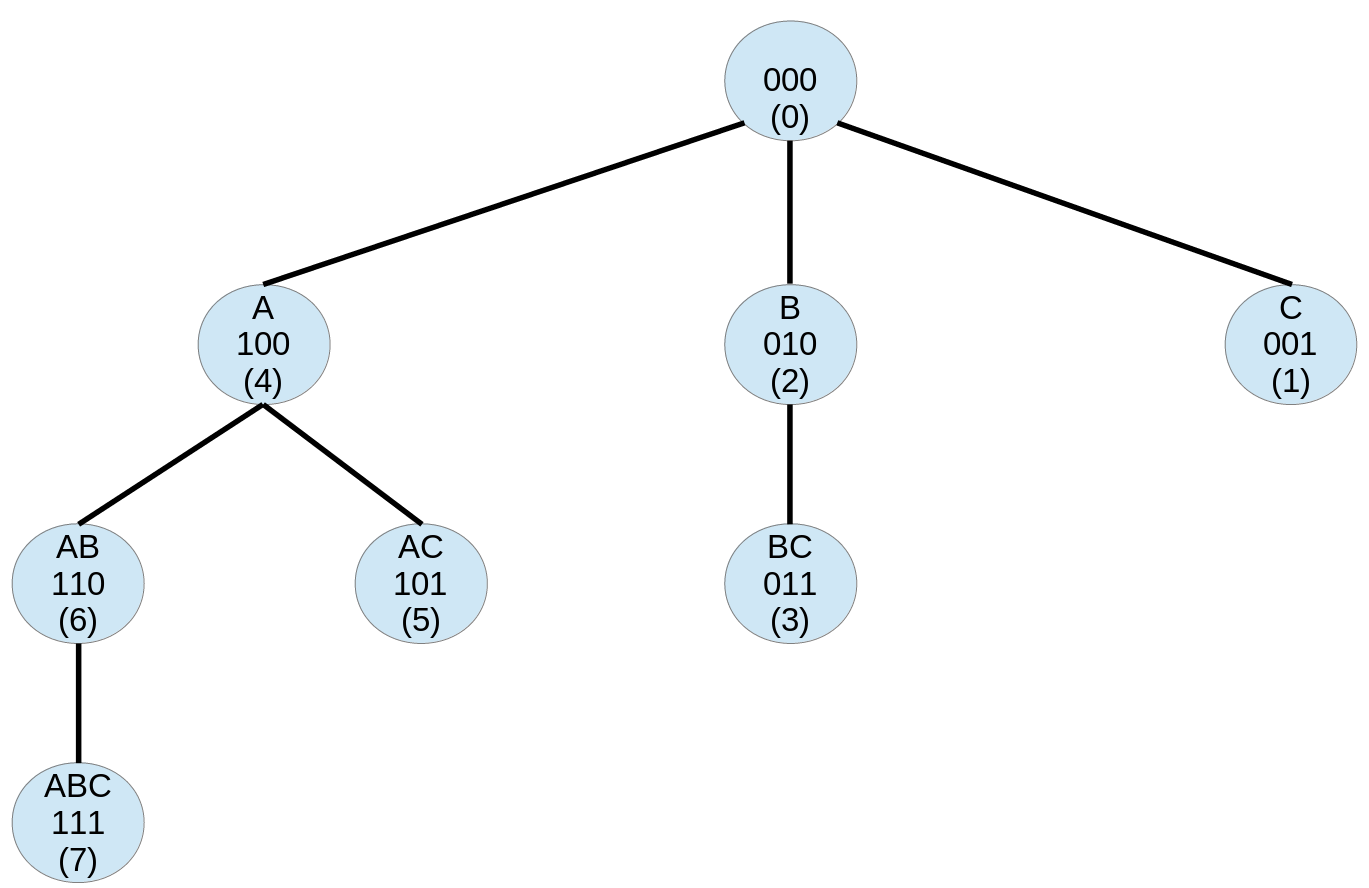
\includegraphics[width=0.7\textwidth]{figs/codificacao}
\caption[Árvore de Combinações Codificada.]
{Árvore de Combinações Codificada.}
\label{fig:codificacao}
\end{figure}

Na Figura \ref{fig:codificacao} é ilustrada uma árvore de combinações para uma rede com $E=\{a,b,c\}$, ou seja, $m=3$. Na imagem, todos os $2^3 = 8$ vértices possuem sua descrição na primeira linha, o valor codificado na base 2 na linha de baixo e o valor convertido para a base 10 entre parênteses na última linha.

\subsection{Decodificação}

Para conhecer os enlaces pertencentes a uma combinação e realizar o teste de viabilidade apropriadamente, é essencial que tal número possa ser decodificado em uma combinação de enlaces. O Algoritmo \ref{alg:decodificador} é usado para decodificar um inteiro em um conjunto de enlaces é apresentado. Vale ressaltar que o processo de decodificação é o responsável por não ser preciso instanciar toda uma árvore de combinações. Com ele, é suficiente conhecer o conjunto de enlaces $E(G)$ e os índices dos {\it bit}s de $B$ para realizar os testes de interferência.

\begin{algorithm}[h]
	\SetVline
	{\bf input:} Número inteiro$B$, número inteiro $I$, conjunto de arestas $E(G)$\\
	$Q \leftarrow B/2$\\
	$R \leftarrow B\%2$\\
	\If{($R=1$)}{
		$C \leftarrow C \cup \{e_I\}$\\
	}
	\If{($Q>0$)}{
		$I \leftarrow I + 1$\\
		DECODIFICADOR(Q, I, E(G))\\
	}
\caption{Algoritmo DECODIFICADOR}
\label{alg:decodificador}
\end{algorithm}

\subsubsection{Prova de Corretude}

O algoritmo apresentado nada mais é do que uma versão recursiva do algoritmo padrão de conversão de um número na base 10 para a base 2 com uma modificação para permitir a captura dos enlaces pertencentes ao conjunto.

Nesse algoritmo, existem duas variáveis de controle, $Q$ e $R$, que são, respectivamente, o quociente e o resto da divisão inteira entre os números $B$ e 2. Se $R=1$, temos $b_I=1$ e, consequentemente, o enlace $e_I$ pertence à combinação $C$ decodificada a partir do inteiro $B$. Reciprocamente, se $b_I=0$, então o enlace $e_I$ não pertence a $C$. A variável $Q$ controla a parada do algoritmo. Enquanto $Q>0$, o processo continua incrementando o valor de $I$ e verificando a pertinência dos enlaces com novos índices $I$. Quando $Q=0$, o processo de conversão é finalizado.

Quando $R=1$, então a condição na linha 3 é satisfeita e o enlace com índice $I$ é adicionado ao conjunto decodificado na linha 4. Portanto, ao final da recursão, $C$ será o conjunto de enlaces decodificado apropriadamente a partir de $B$.

\subsubsection{Análise de Complexidade}

Todas as linhas do algoritmo são $O(1)$. Contudo, como trata-se de um algoritmo recursivo, a função DECODIFICADOR será chamada o número de vezes equivalente ao índice do {\it bit} ativo mais significativo. No pior caso, teremos $m-1$ chamadas da função, o que define sua complexidade de tempo como $O(m)$. Para o processo de decodificação é preciso armazenar, no máximo, $m-1$ enlaces e, portanto, sua complexidade de espaço é O(m).

\section{Percorrendo a Árvore Iterativamente}
\label{section:busca-iterativa}

No exemplo da Figura 3.1, foi visto que, para uma rede com $4$ enlaces, tem-se uma árvore de combinações com $16$ vértices. A árvore é estruturada da raiz ($C=\varnothing$ ou $B=0$) à sua folha de maior altura ($C=E$ ou $B=15$). De forma geral, para um grafo com $m$ enlaces, a árvore possui $2^m$ vértices, partindo de $B=0$ e chegando a $B=2^m-1$.

Na árvore codificada, a ordem em que os enlaces são considerados é muito importante porque os índices dos {\it bit}s de $B$ são estritamente relacionados aos enlaces $e$, consequentemente, cada combinação $C$ é codificada unicamente por um número inteiro $B$.

Sabendo disso, é possível percorrer a árvore de combinações simplesmente realizando uma contagem que vai de 0 até $2^m -1$. Ou seja, todo vértice codificado $B>0$ é alcançado a partir da soma de um outro nó codificado mais $1$.

\begin{figure}[htb]
\centering
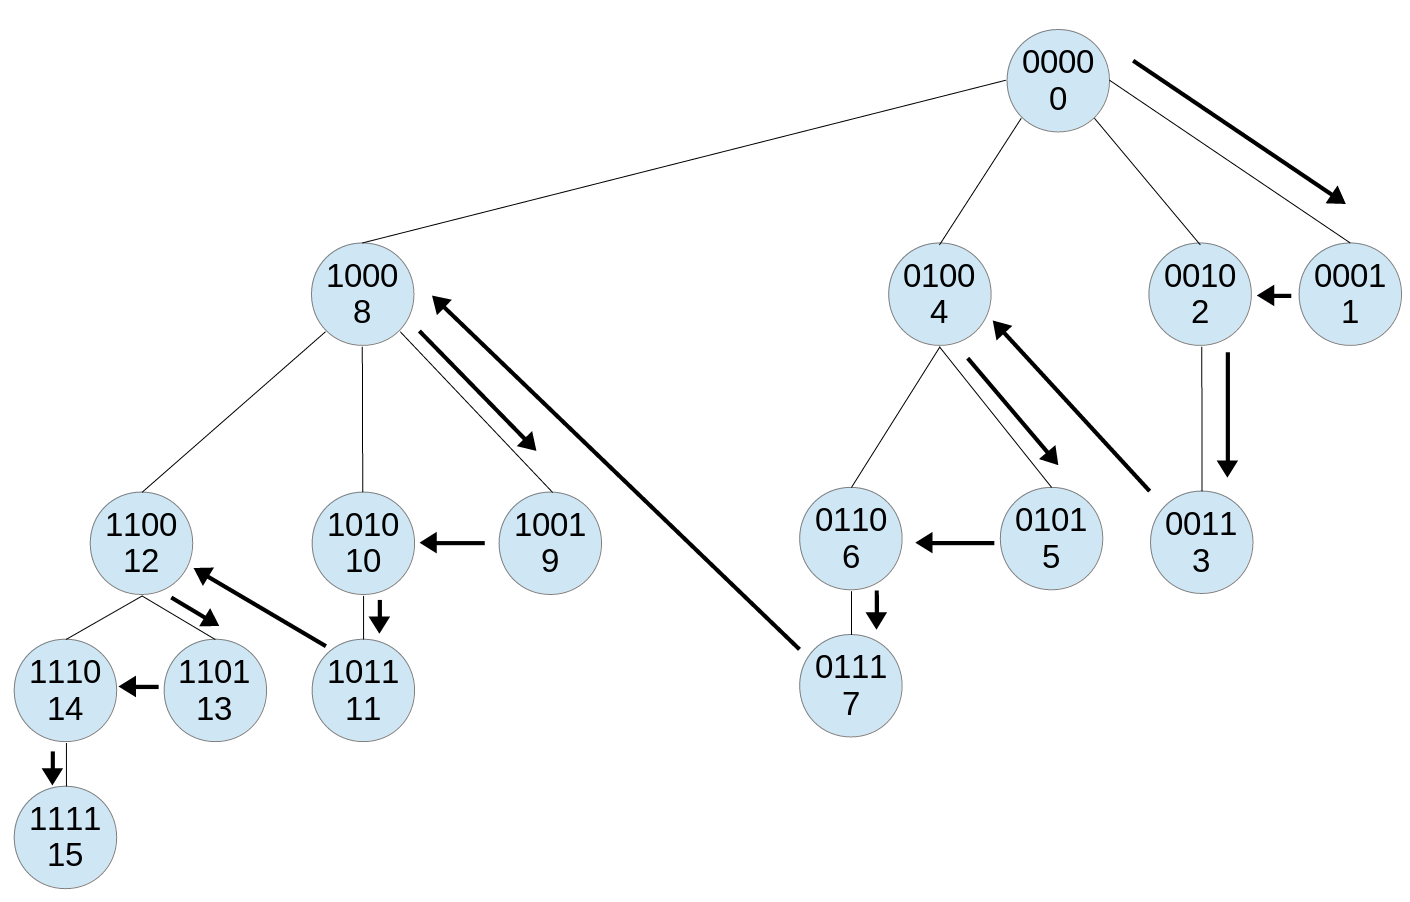
\includegraphics[width=0.7\textwidth]{figs/buscaiterativa}
\caption[Busca Iterativa (Contagem).]
{Busca Iterativa (Contagem).}
\label{fig:buscaiterativa}
\end{figure}

A Figura \ref{fig:buscaiterativa} mostra como a árvore do exemplo anterior é percorrida através da contagem. Comparado com o método de busca adotado no capítulo anterior, é importante ressaltar que a ordem em que os vértices são visitados é totalmente diferente. Essa nova ordem é consistente com uma contagem que somente é alcançável devido a codificação aqui introduzida.

\section{``Podando'' a Árvore de Combinações}
\label{section:saltos}

Diferente do caso anterior, a vantagem em codificar as combinações para a atividade de ``poda'' da árvore não é tão trivial. Contudo, o método de busca baseado na contagem será usado para detectar alguns padrões que ajudam a ``podar'' a árvore de maneira eficiente. Mais uma vez, a correspondência entre $E$ e $B$ é muito importante e sua ordem, uma vez ar{\it bit}rada, deve ser mantida no decorrer do processo. 

Dado um inteiro $B$, seus {\it bit}s $b_i$ podem fornecer mais informações úteis além da pertinência do enlace $e_i$ ao conjunto $C$. Considere o caso em que $b_i^*$ é o {\it bit} ativo menos significativo, ou seja, é o {\it bit} 1 mais à direita. Nesse caso, o índice $i$ de $b_i^*$ também representa o número de filhos que $B$ tem na árvore, ou seja, quantas combinações são descendentes diretos, de $C$. Em termos de {\it bit}s, $i$ representa os números que são resultantes da variação dos {\it bit}s 0 à direita de $b_i^*$ em $B$.

Isso significa que $b_i^*$ tem muito a dizer sobre os descendentes de $B$. Especificamente, se essa ideia for aplicada de maneira recursiva aos filhos $B'$ de $B$, seus $b_i^*$’s vão indicar o número de netos de $B$ e assim por diante. Ao final da recursão, uma combinação $C$ que foi codificada em $B$ tal que $b_i^*$ é o {\it bit} ativo menos significativo tem exatamente $2^i–1$ descendentes na árvore.

No Capítulo \ref{cap:modelagem}, baseado na ideia de inviabilidade hereditária, o termo ``podar'' a árvore foi definido como o ato de ignorar os descendentes de uma combinação não viável ao percorrer uma árvore. Para o presente caso, como uma contagem está sendo feita, um termo mais adequado seria ``saltar''. Portanto, uma vez que uma combinação codificada $B$ não for viável, um ``salto'' na contagem será realizado sobre todos os seus descendentes.

Como o número de descendentes de uma combinação B é facilmente determinável usando $b_i^*$, caso seja necessário realizar um ``salto'' na contagem devido a inviabilidade de $B$, basta incrementar a contagem com o número de descendentes mais $1$. Ou seja, se $B$ não é viável, a próxima combinação a ser testada será $B + 2^i$, onde $i$ é o índice do {\it bit} ativo menos significativo.

\begin{figure}[htb]
\centering
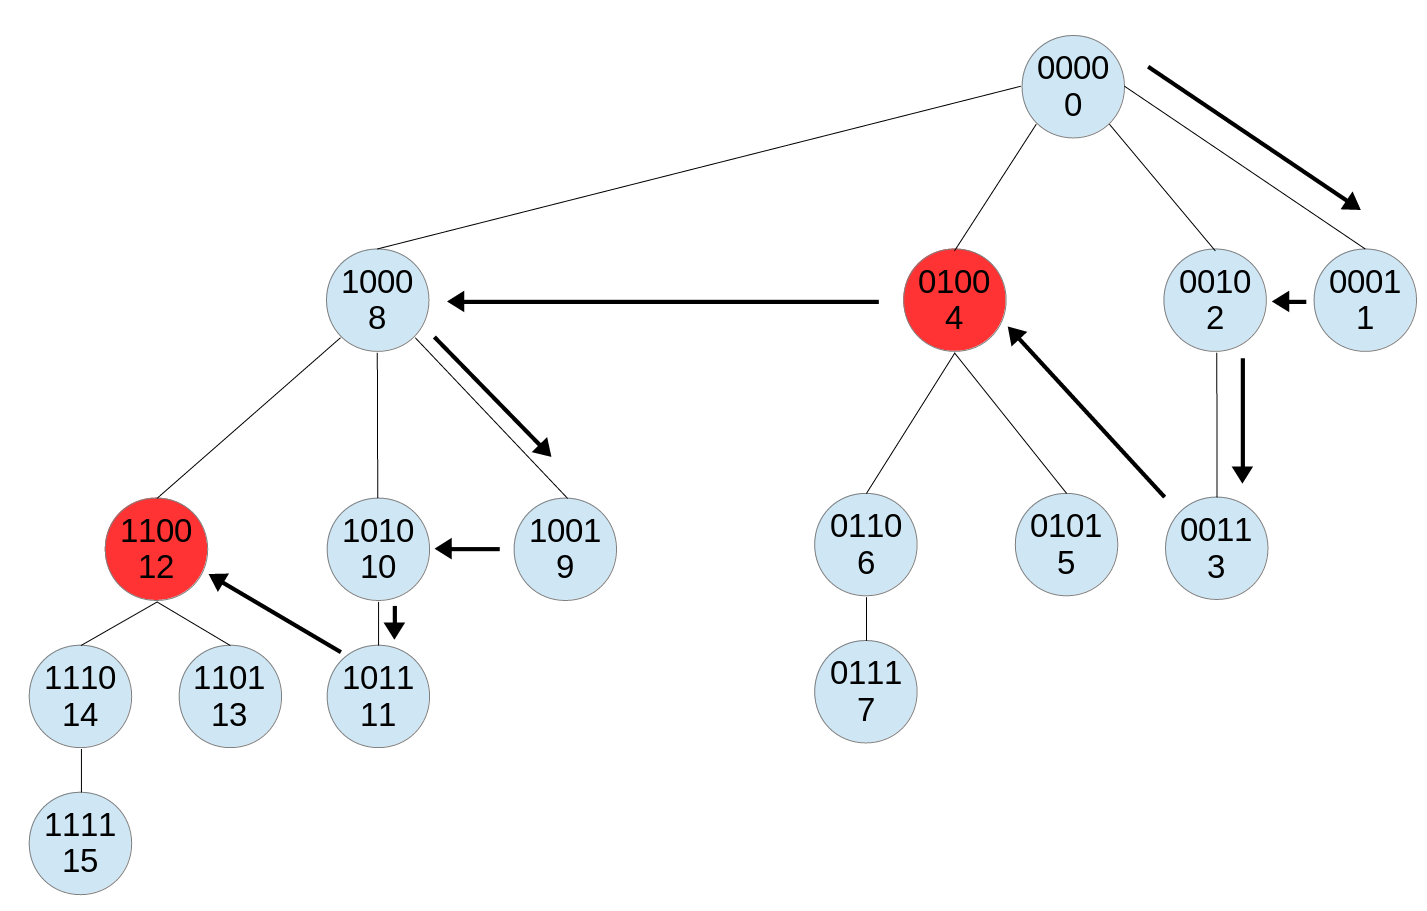
\includegraphics[width=0.7\textwidth]{figs/saltos}
\caption[Exemplo de ``saltos'' na Contagem.]
{Exemplo de ``saltos'' na Contagem.}
\label{fig:saltos}
\end{figure}

Um exemplo de cenário em que os ``saltos'' ocorrem é ilustrado na Figura \ref{fig:saltos}. Na rede do exemplo, sabe-se que as combinações $4$ e $12$ não são viáveis. Por isso, todos os descendentes de $4$ e de $12$ serão ignorados na contagem, resultando na sequência $0, 1, 2, 3, 4, 8, 9, 10, 11, 12$. Até esse ponto, as combinações de enlaces viáveis ainda não estão sendo listadas, apenas está sendo mostrada a sequência de enlaces visitados na contagem.

\section{Algoritmo Iterativo para Enumeração de Conjuntos de Enlaces Viáveis}
\label{section:iterativo}

Finalmente, agora que os métodos de como percorrer a árvore de combinações, ``saltar'' sobre os descendentes das combinações inviáveis e decodificar os inteiros para realizar os testes de interferência são conhecidos, é possível descrever o algoritmo iterativo para enumeração de conjuntos de enlaces viáveis.

\begin{algorithm}[h]
	\SetVline
	{\bf input:} Grafo direcionado $G=(V,E)$\\
	{\bf output:} Conjuntos de Enlaces Viáveis $F$\\
	$F \leftarrow \varnothing$\\
	$C \leftarrow \varnothing$\\
	$B \leftarrow 0$\\
	$I \leftarrow 0$\\
	\While{$B<2^m$}{
		$C \leftarrow DECODIFICADOR(B, 0, E(G))$\\
		\If{$VIAVEL(C)$}{
			$F \leftarrow F \cup {B}$\\
			$I \leftarrow 1$\\
		}
		\Else{
			$I \leftarrow 2^{i*}$\\
		}
		$B \leftarrow B + I$\\
	}
\caption{Algoritmo ITERATIVO}
\label{alg:iterativo}
\end{algorithm}

\subsubsection{Prova de Corretude}

De acordo com o que foi provado na Seção \ref{section:busca}, o laço instanciado na linha 7 e o incremento feito na linha 14 representam uma contagem e, de fato, fazem o algoritmo percorrer todas as combinações de enlaces. Caso uma combinação seja viável, ela passará no teste da linha 9 e será adicionada ao resultado final na linha 10.

Os ``saltos'' demonstrados na Seção \ref{section:saltos} são baseados na variável $I$, usada como incremento à variável $B$. Pelo algoritmo, $I$ somente possui dois valores possíveis. 

\[ I =
\begin{cases}
	1	& \quad	\text{se, e somente se, } B \text{ é viável} \\
	2^{i*}	& \quad	\text{caso contrário} \\
  \end{cases}
\]

Essa seleção de valores é gerenciada pela condicional das linhas 9 e 12.

Devido a inviabilidade hereditária, todos os $2^{i*}$ descendentes de uma combinação inviável certamente também são inviáveis. Portanto, os ``saltos'' apenas tem o papel de agilizar o processo e não interferem no resultado final do algoritmo.

Conclui-se que, de fato, o algoritmo retorna todos os conjuntos de enlaces viáveis e, portanto, está correto.

\subsubsection{Análise de Complexidade}

O processo de decodificação apresentado é responsável por tornar desnecessário o armazenamento de todas as combinações de enlaces possíveis, como precisava ser feito na abordagem do capítulo anterior. Portanto, a complexidade de espaço é reduzida de $O(2^m)$ para $O(m)$.

	As linhas 1-4, 7-12 são $O(1)$. A função de decodificação na linha 6 é $O(m)$ e o teste de viabilidade na linha 7 é $O(m^2)$. O laço principal das linhas 5-12 é $O(2^mm^2)$ pois a cada uma das $2^m$ iterações (no pior caso), a função de decodificação e o teste de viabilidade são chamados com complexidade de $O(m) + O(m^2) = O(m^2)$. De maneira geral, a complexidade de tempo total é  $O(2^mm^2)$. 

Analogamente ao que foi explicado no capítulo anterior, esse valor de complexidade é muito exagerado e também cabe fazer a substituição de $2^m$ por $|F|$. Portanto, a complexidade é $O(|F|m^2)$.

\section{Conclusão}
\label{section:conclusao3}

Nesse capítulo, uma ideia de como percorrer a árvore em busca de combinações viáveis foi formalizada na forma de um algoritmo iterativo. Diferente da abordagem do capítulo anterior, devido ao processo de decodificação, apenas o conjunto de enlaces precisa ser armazenado, reduzindo consideravelmente sua complexidade de espaço. Contudo, sua complexidade de tempo continua a mesma do caso anterior.
